\begin{SCn}
	
\scnsectionheader{\currentname}
\scnstartsubstruct

\scnheader{Предметная область программных вариантов реализации базового интерпретатора логико-семантических моделей ostis-систем на современных компьютерах}
\scnsdmainclasssingle{программный вариант реализации платформы интерпретации sc-моделей компьютерных систем}
\scnsdclass{***}

\scnheader{программный вариант реализации платформы интерпретации sc-моделей компьютерных систем}
\scnidtf{программный вариант реализации базового интерпретатора логико-семантических моделей компьютерных систем}
\scnidtf{программный вариант реализации базового интерпретатора логико-семантических моделей ostis-систем на современных компьютерах}
\scnidtf{вариант реализации базового интерпретатора логико-семантических моделей компьютерных систем на традиционных компьютерах с архитектурой фон Неймана}
\scnexplanation{Одним из путей, позволяющих осуществлять апробацию, развитие, а в ряде случаев и внедрение новых моделей и технологий вне зависимости от наличия соответствующих аппаратных средств является разработка программных моделей этих аппаратных средств, которые были бы функционально эквивалентны этим аппаратным средствам, но при этом интерпретировались на базе традиционной аппаратной архитектуры (в данной работе традиционной архитектурой будем считать архитектуру фон Неймана, как доминирующую в настоящее время). Очевидно, что производительность таких программных моделей в общем случае будет ниже, чем самих аппаратных решений, однако в большинстве случаев она оказывается достаточной для того, чтобы развивать соответствующую технологию параллельно с разработкой аппаратных средств и осуществления постепенного перевода уже работающих систем с программной модели на аппаратные средства.}
\scnsuperset{web-ориентированный вариант реализации платформы интерпретации sc-моделей компьютерных систем}
\scnaddlevel{1}
	\scnidtf{вариант реализации платформы интерпретации sc-моделей компьютерных систем предполагающий взаимодействие пользователей с системой посредством сети Интернет}
	\scnsubset{многопользовательский вариант реализации платформы интерпретации sc-моделей компьютерных систем}
	\scnhaselement{Программный вариант реализации платформы интерпретации sc-моделей компьютерных систем}
\scnaddlevel{-1}

\scnheader{Программный вариант реализации платформы интерпретации sc-моделей компьютерных систем}
\scntext{принципы реализации}{Поскольку sc-тексты представляют собой семантические сети, то есть, по сути, графовые конструкции определенного вида, то на нижнем уровне задача разработки программного варианта реализации платформы интерпретации sc-моделей сводится к разработке средств хранения и обработки таких графовых конструкций.
	
	К настоящему времени разработано большое количество простейших моделей представления графовых конструкций в линейной памяти, таких как матрицы смежности, списки смежности и другие \scncite{Diskrete_Math}. Однако, при разработке сложных систем как правило приходится использовать более эффективные модели, как с точки зрения объема информации, требуемого для представления, так и с точки зрения эффективности обработки графовых конструкций, хранимых в той или иной форме.
	
	К наиболее распространенным программным средствам, ориентированным на хранение и обработку графовых конструкций относятся графовые СУБД (Neo4j \scncite{Neo4j}, ArangoDB \scncite{ArangoDB}, OrientDB \scncite{OrientDB}, Grakn \scncite{Grakn} и др.), а также так называемые rdf-хранилища (Virtuoso \scncite{Virtuoso}, Sesame \scncite{Sesame} и др.), предназначенные для хранения конструкций, представленных в модели RDF. Для доступа к информации, хранимой в рамках таких средств, могут использоваться как языки, реализуемые в рамках конкретного средства (например, язык Cypher в Neo4j), так и языки, являющиеся стандартами для большого числа систем такого класса (например, SPARQL для rdf-хранилищ).
	
	Популярность и развитость такого рода средств приводит к тому, что на первый взгляд целесообразным и эффективным кажется вариант реализации \textit{программного варианта реализации платформы интерпретации sc-моделей} на базе одного из таких средств. Однако, существует ряд причин, по которым было принято решение о реализации \textit{программного варианта реализации платформы интерпретации sc-моделей} с нуля. К ним относятся следующие:
	
	\begin{scnitemize}
		\item для обеспечения эффективности хранения и обработки информационных конструкций определенного вида (в данном случае -- конструкций SC-кода, sc-конструкций), должна учитываться специфика этих конструкций. В частности, описанные в работе \scncite{Koronchik2013} эксперименты показали значительный прирост эффективности собственного решения по сравнению с существующими на тот момент;
		\item в отличие от классических графовых конструкций, где дуга или ребро могут быть инцидентны только вершине графа (это справедливо и для rdf-графов) в SC-коде вполне типичной является ситуация, когда sc-коннектор инцидентен другому sc-коннектору или даже двум sc-коннекторам. В связи с этим существующие средства хранения графовых конструкций не позволяют в явном виде хранить sc-конструкции (sc-графы). Возможным решением данной проблемы является переход от sc-графа к орграфу инцидентности, пример которого описан в работе \scncite{Ivashenko2015}, однако такой вариант приводит к увеличению числа хранимых элементов в несколько раз и значительно снижает эффективность алгоритмов поиска из-за необходимости делать большое количество дополнительных итераций;
		\item в основе обработки информации в рамках Технологии OSTIS лежит многоагентный подход, в рамках которого агенты обработки информации, хранимой в sc-памяти (sc-агенты) реагируют на события, происходящие в sc-памяти и обмениваются информацией посредством спецификации выполняемых ими действий в sc-памяти \scncite{Shunkevich2018}. В связи с этим одной из важнейших задач является реализация в рамках \textit{программного варианта реализации платформы интерпретации sc-моделей} возможности подписки на события, происходящие в программной модели sc-памяти, которая на данный момент практически не поддерживается в рамках современных средств хранения и обработки графовых конструкций;
		\item SC-код позволяет описывать также внешние информационные конструкции любого рода (изображения, текстовые файла, аудио- и видеофайлы и т.д.), которые формально трактуются как содержимое \textit{sc-элементов}, являющихся знаками \textit{внешних файлов ostis-системы}. Таким образом, компонентом \textit{программного варианта реализации платформы интерпретации sc-моделей} должна быть реализация файловой памяти, которая позволяет хранить указанные конструкции в каких-либо общепринятых форматах. Реализация такого компонента в рамках современных средств хранения и обработки графовых конструкций также не всегда представляется возможной.
	\end{scnitemize}
	
	По совокупности перечисленных причин было принято решение о реализации \textit{программного варианта реализации платформы интерпретации sc-моделей} "с нуля"{} с учетом особенностей хранения и обработки информации в рамках Технологии OSTIS.}
\scnrelfromset{декомпозиция программной системы}{Программная модель sc-памяти;Реализация интерпретатора sc-моделей пользовательских интерфейсов}
\scnexplanation{Текущий \textit{Программный вариант реализации платформы интерпретации sc-моделей компьютерных систем} является web-ориентированным, то есть с точки зрения современной архитектуры каждая ostis-система представляет собой web-сайт доступный онлайн посредством обычного браузера. Такой вариант реализации обладает очевидным преимуществом -- доступ к системе возможен из любой точки мира, где есть Интернет, при этом для работы с системой не требуется никакого специализированного программного обеспечения. С другой стороны, такой вариант реализации обеспечивает возможность параллельной работы с системой нескольких пользователей.

В то же время, взаимодействие клиентской и серверной части организовано таким образом, что web-интерфейс может быть легко заменен на настольный или мобильный интерфейс, как универсальный, так и специализированный.

Данный вариант реализации распространяется под open-source лицензией, для хранения исходных текстов используется хостинг Github и коллективная учетная запись ostis-dev.

Реализация является кроссплатформенной и может быть собрана из исходных текстов в различных операционных системах.}
\scnrelfrom{иллюстрация}{\scnfileimage{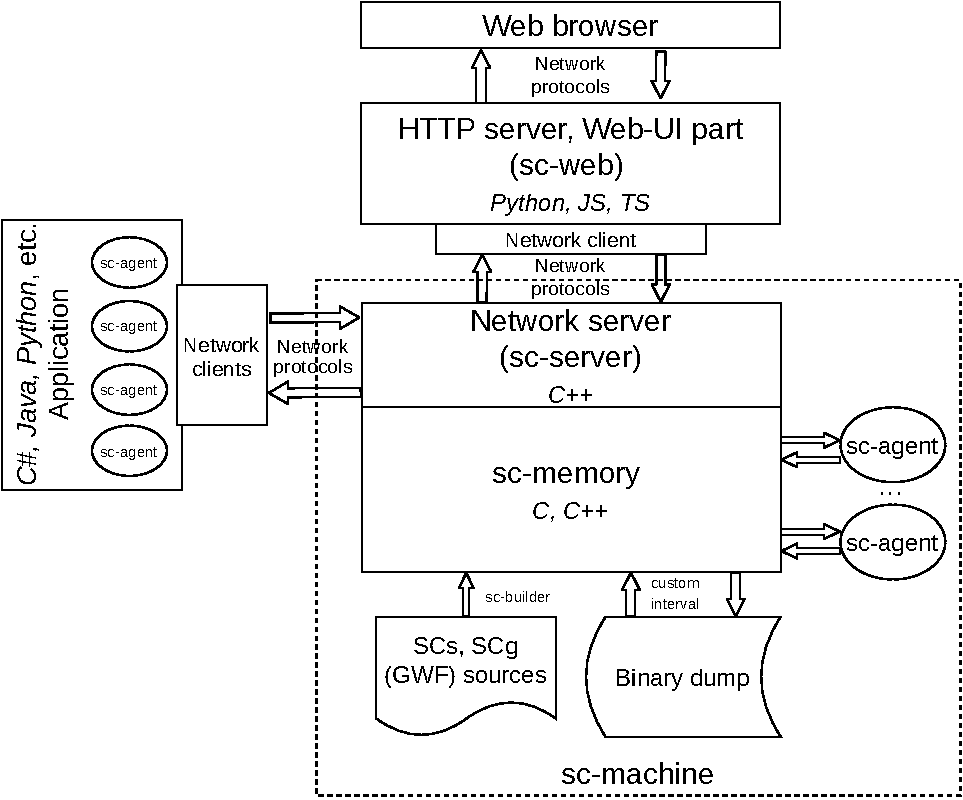
\includegraphics[scale=0.95]{figures/sd_interpreters/platform-ostis-architecture.pdf}}}
\scnaddlevel{1}
	\scnexplanation{На приведенной иллюстрации видно, что ядром платформы является \textit{Программная модель sc-памяти} (sc-machine), которая одновременно может взаимодействовать как с \textit{Реализацией интерпретатора sc-моделей пользовательских интерфейсов} (sc-web \scncite{sc_web}), так и с любыми сторонними приложениями по соответствующим сетевым протоколам. С точки зрения общей архитектуры \textit{Реализация интерпретатора sc-моделей пользовательских интерфейсов} выступает как один из множества возможных внешних компонентов, взаимодействующих с \textit{Программной моделью sc-памяти} по сети.}
\scnaddlevel{-1}

\scnheader{Программная модель sc-памяти}
\scnidtf{sc-machine}
\scnidtf{Программная модель семантической памяти, реализованная на основе традиционной линейной памяти и включающая средства хранения sc-конструкций и базовые средства для обработки этих конструкций, в том числе удаленного доступа к ним посредством соответствующих сетевых протоколов}
\scnrelto{программная модель}{sc-память}
\scniselement{программная модель sc-памяти на основе линейной памяти}
\scntext{основной репозиторий исходных текстов}{https://github.com/ostis-dev/sc-machine.git}
\scnrelfromlist{компонент программной системы}{Реализация sc-хранилища и средств доступа к нему\\
	\scnaddlevel{1}
		\scnexplanation{В рамках текущей \textit{Программной модели sc-памяти} под \textit{sc-хранилищем} понимается компонент программной модели, осуществляющий хранение sc-конструкций и доступ к ним через программный интерфейс. В общем случае \textit{sc-хранилище} может быть реализовано по-разному. Кроме собственно \textit{sc-хранилища} \scnbispace \textit{Программная модель sc-памяти} включает также \textit{Реализацию файловой памяти ostis-системы}, предназначенную для хранения содержимого \textit{внутренних файлов ostis-систем}. Стоит отметить, что при переходе с \textit{Программной модели sc-памяти} на ее аппаратную реализацию файловую память ostis-системы целесообразно будет реализовывать на основе традиционной линейной памяти (во всяком случае, на первых этапах развития \textit{семантического компьютера}).}
	\scnaddlevel{-1}
	;Реализация базового набора платформенно-зависимых sc-агентов и их общих компонентов;Реализация подсистемы взаимодействия с внешней средой с использованием сетевых протоколов;Реализация вспомогательных инструментальных средств для работы с sc-памятью;Реализация scp-интерпретатора}
\scntext{программная документация}{http://ostis-dev.github.io/sc-machine/}
\scnrelfromlist{используемый язык программирования}{C;C++;Python}
\scnnote{Текущий вариант \textit{Программной модели sc-памяти} предполагает возможность сохранения состояния (слепка) памяти на жесткий диск и последующей загрузки из ранее сохраненного состояния. Такая возможность необходима для перезапуска системы, в случае возможных сбоев, а также при работе с исходными текстами базы знаний, когда сборка из исходных текстов сводится к формированию слепка состояния памяти, который затем помещается в \textit{Программную модель sc-памяти}.}

\scnheader{Реализация sc-хранилища и средств доступа к нему}
\scnrelfromlist{компонент программной системы}{Реализация sc-хранилища;Реализация файловой памяти ostis-системы}

\scnheader{Реализация sc-хранилища}
\scniselement{реализация sc-хранилища на основе линейной памяти}
\scnrelfrom{иллюстрация}{\scnfileimage{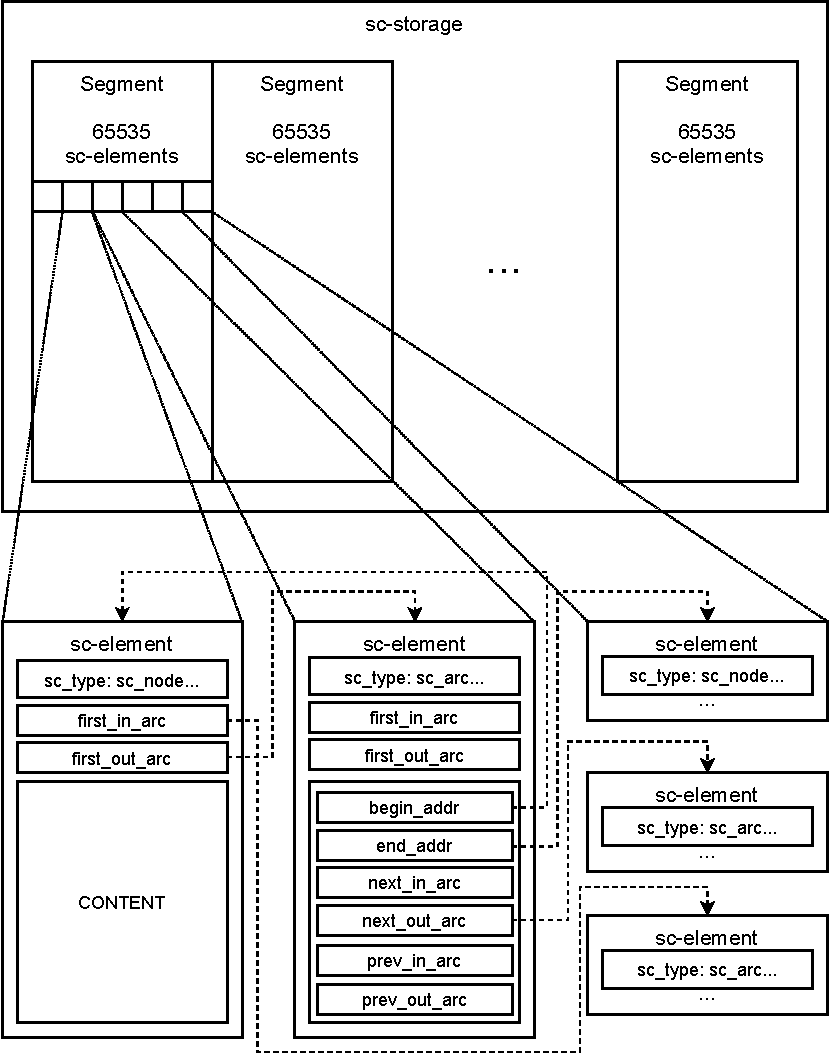
\includegraphics{figures/sd_interpreters/sc-storage.pdf}}}
\scnrelfrom{класс объектов программной системы}{сегмент sc-хранилища}
\scnaddlevel{1}
	\scnidtf{страница sc-хранилища}
	\scnexplanation{В рамках данной реализации \textit{sc-хранилища} \scnbigspace \textit{sc-память} моделируется в виде набора \textit{сегментов}, каждый из которых представляет собой фиксированного размера упорядоченную последовательность \textit{элементов sc-хранилища}, каждый из которых соответствует конкретному sc-элементу. В настоящее время каждый сегмент состоит из $2^{16}-1=65535$ \textit{элементов sc-хранилища}. Выделение \textit{сегментов sc-хранилища} позволяет, с одной стороны, упростить адресный доступ к \textit{элементам sc-хранилища}, с другой стороны -- реализовать возможность выгрузки части sc-памяти из оперативной памяти на файловую систему при необходимости. Во втором случае сегмент sc-хранилища становится минимальной (атомарной) выгружаемой частью sc-памяти. Механизм выгрузки сегментов реализуется в соответствии с существующими принципами организации виртуальной памяти в современных операционных системах.}
	\scnnote{Максимально возможное число сегментов ограничивается настройками программной реализации sc-хранилища (в настоящее время по умолчанию установлено количество $2^{16}-1=65535$ сегментов, но в общем случае оно может быть другим). Таким образом, технически максимальное количество хранимых sc-элементов в текущей реализации составляет около $4.3 \times 10^{9}$ sc-элементов.}
	\scnnote{По умолчанию все сегменты физически располагаются в оперативной памяти, если объема памяти не хватает, то предусмотрен механизм выгрузки части сегментов на жесткий диск (механизм виртуальной памяти).}
	\scnrelfrom{класс объектов программной системы}{элемент sc-хранилища}
		\scnaddlevel{1}
			\scnexplanation{Каждый сегмент состоит из набора структур данных, описывающих конкретные \textit{sc-элементы} (элементов sc-хранилища). Независимо от типа описываемого sc-элемента каждый \textit{элемент sc-хранилища} имеет фиксированный размер (в текущий момент -- 48 байт), что обеспечивает удобство их хранения. Таким образом, максимальный размер базы знаний в текущей программной модели sc-памяти может достигнуть 223 Гб (без учета содержимого \textit{внутренних файлов ostis-системы}, хранимого на внешней файловой системе).}
		\scnaddlevel{-1}
\scnaddlevel{-1}
\scnrelfrom{пример}{\scnfileimage{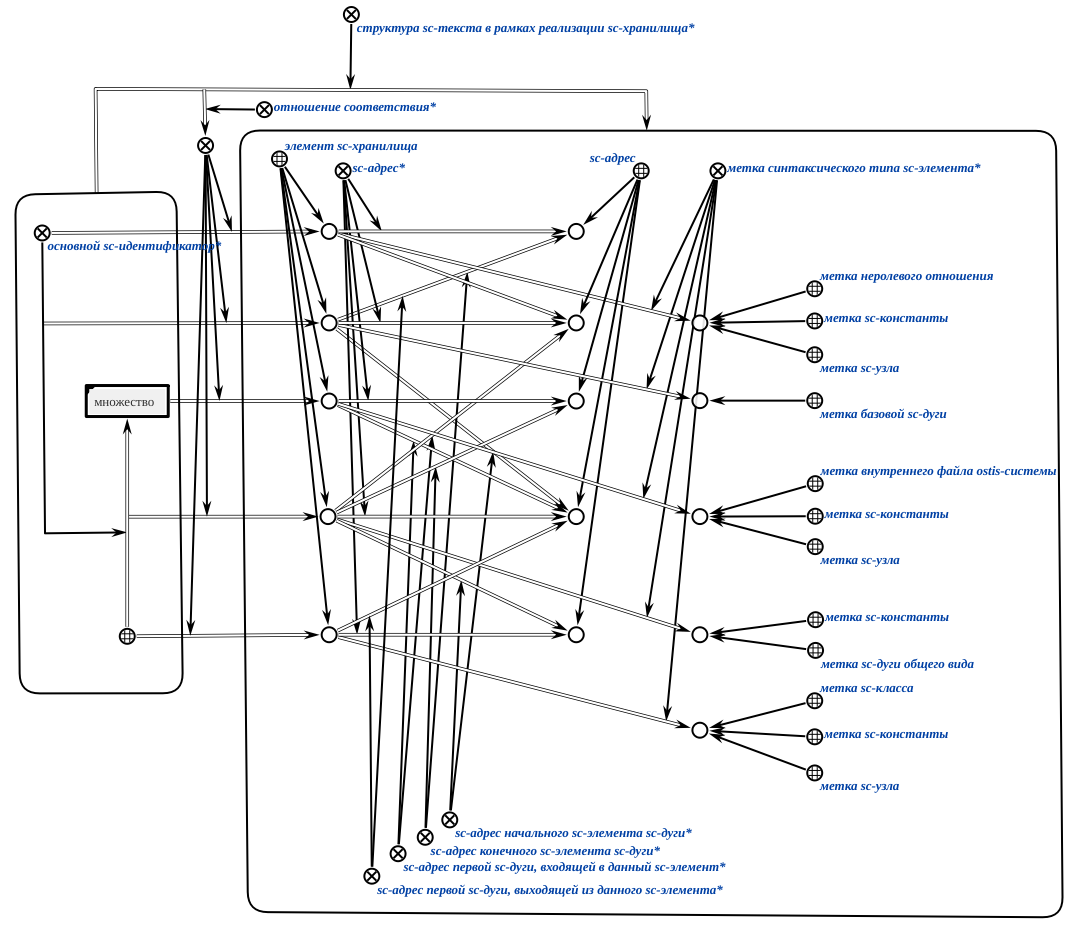
\includegraphics[scale=0.6]{figures/sd_interpreters/storage_example.png}}}
\scnaddlevel{1}
	\scnnote{Для наглядности в данном примере опущены \textit{метки уровня доступа}}
\scnaddlevel{-1}

\scnheader{sc-адрес}
\scnidtf{адрес элемента sc-хранилища, соответствующего заданному sc-элементу, в рамках текущего состояния реализации sc-хранилища в составе программной модели sc-памяти}
\scnexplanation{Каждый элемент sc-хранилища в текущей реализации может быть однозначно задан его адресом (sc-адресом), состоящим из номера сегмента и номера \textit{элемента sc-хранилища} в рамках сегмента. Таким образом, \textit{sc-адрес} служит уникальными координатами \textit{элемента sc-хранилища} в рамках \textit{Реализации sc-хранилища}.}
\scnnote{Sc-адрес никак не учитывается при обработке базы знаний на семантическом уровне и необходим только для обеспечения доступа к соответствующей структуре данных, хранящейся в линейной памяти на уровне \textit{Реализации sc-хранилища}.}
\scnnote{В общем случае sc-адрес элемента sc-хранилища, соответствующего заданному sc-элементу, может меняться, например, при пересборке базы знаний из исходных текстов и последующем перезапуске системы. При этом sc-адрес элемента sc-хранилища, соответствующего заданному sc-элементу, непосредственно в процессе работы системы в текущей реализации меняться не может.}
\scnnote{Для простоты будем говорить "sc-адрес sc-элемента"{}, имея в виду \textit{sc-адрес} \scnbigspace \textit{элемента sc-хранилища}, однозначно соответствующего данному \textit{sc-элементу}.}
\scnrelfromlist{семейство отношений, однозначно задающих структуру заданной сущности}{номер сегмента sc-хранилища*;номер элемента sc-хранилища в рамках сегмента*}

\scnheader{элемент sc-хранилища}
\scnidtf{ячейка sc-хранилища}
\scnidtf{элемент sc-хранилища, соответствующий sc-элементу}
\scnidtf{образ sc-элемента в рамках sc-хранилища}
\scnidtf{структура данных, каждый экземпляр которой соответствует одному sc-элементу в рамках sc-хранилища}
\scnexplanation{Каждый элемент sc-хранилища, соответствующий некоторому sc-элементу, описывается его синтаксическим типом (меткой), а также независимо от типа указывается sc-адрес первой входящей в данный sc-элемент sc-дуги и первой выходящей из данного sc-элемента sc-дуги (могут быть пустыми, если таких sc-дуг нет). 
	
Оставшиеся байты в зависимости от типа соответствующего sc-элемента (sc-узел или sc-дуга) могут использоваться либо для хранения содержимого внутреннего файла ostis-системы (может быть пустым, если sc-узел не является знаком файла), либо для хранения спецификации sc-дуги.}
\scnsubdividing{элемент sc-хранилища, соответствующий sc-узлу\\
	\scnaddlevel{1}
		\scnrelfromset{семейство отношений, однозначно задающих структуру заданной сущности}{метка синтаксического типа sc-элемента*;метка уровня доступа sc-элемента*;sc-адрес первой sc-дуги, выходящей из данного sc-элемента*;sc-адрес первой sc-дуги, входящей в данный sc-элемент*;содержимое элемента sc-хранилища*\\
		\scnaddlevel{1}
			\scnrelfrom{второй домен}{содержимое элемента sc-хранилища}
			\scnaddlevel{1}
				\scnidtf{содержимое элемента sc-хранилища, соответствующего внутреннему файлу ostis-системы}
			\scnaddlevel{-1}
			\scnexplanation{Каждый sc-узел в текущей реализации может иметь содержимое (может стать \textit{внутренним файлом ostis-системы}).
			В случае, если размер содержимого внутреннего файла ostis-системы не превышает 48 байт (размер \textit{спецификации sc-дуги в рамках sc-хранилища}, например небольшой \textit{строковый sc-идентификатор}), то это содержимое явно хранится в рамках элемента sc-хранилища в виде последовательности байт.
			В противном случае оно помещается в специальным образом организованную файловую память (за ее организацию отвечает отдельный модуль платформы, который в общем случае может быть устроен по-разному), а в рамках элемента sc-хранилища хранится уникальный адрес соответствующего файла, позволяющий быстро найти его на файловой системе.}
		\scnaddlevel{-1}}
		\scnaddlevel{1}
			\scnnote{\textit{sc-адрес первой sc-дуги, выходящей из данного sc-элемента*}, \textit{sc-адрес первой sc-дуги, входящей в данный sc-элемент*} и \textit{содержимое элемента sc-хранилища*} в общем случае могут отсутствовать (быть нулевыми, "пустыми"{}), но размер элемента в байтах останется тем же.}
		\scnaddlevel{-1}
	\scnaddlevel{-1}
	;элемент sc-хранилища, соответствующий sc-дуге\\
	\scnaddlevel{1}
	\scnrelfromset{семейство отношений, однозначно задающих структуру заданной сущности}{метка синтаксического типа sc-элемента*;метка уровня доступа sc-элемента*;sc-адрес первой sc-дуги, выходящей из данного sc-элемента*;sc-адрес первой sc-дуги, входящей в данный sc-элемент*;спецификация sc-дуги в рамках sc-хранилища*\\
		\scnaddlevel{1}
			\scnrelfrom{второй домен}{спецификация sc-дуги в рамках sc-хранилища}
			\scnaddlevel{1}
			\scnrelfromset{семейство отношений, однозначно задающих структуру заданной сущности}{sc-адрес начального sc-элемента sc-дуги*;sc-адрес конечного sc-элемента sc-дуги*;sc-адрес следующей sc-дуги, выходящей из того же sc-элемента*;sc-адрес следующей sc-дуги, входящей в тот же sc-элемент*;sc-адрес предыдущей sc-дуги, выходящей из того же sc-элемента*;sc-адрес предыдущей sc-дуги, входящей в тот же sc-элемент*}
			\scnaddlevel{-1}
		\scnaddlevel{-1}}
	\scnnote{sc-ребра в текущий момент хранятся так же, как sc-дуги, то есть имеют начальный и конечный sc-элементы, отличие заключается только в \textit{метке синтаксического типа sc-элемента}. Это приводит к ряду неудобств при обработке, но sc-ребра используются в настоящее время достаточно редко.}
	\scnaddlevel{-1}}
\scnaddlevel{1}
	\scnnote{С точки зрения программной реализации структура данных для хранения sc-узла и sc-остается остается та же, но в ней меняется список полей (компонентов).\\
	Кроме того, как можно заметить каждый элемент sc-хранилища (в том числе, \textit{элемент sc-хранилища, соответствующий sc-дуге}) не хранит список sc-адресов связанных с ним sc-элементов, а хранит sc-адреса одной выходящей и одной входящей дуги, каждая из которых в свою очередь хранит sc-адреса следующей и предыдущей дуг в списке исходящих и входящих sc-дуг для соответствующих элементов.\\
	Все перечисленное позволяет:
	\begin{scnitemize}	
		\item сделать размер такой структуры фиксированным (в настоящее время 48 байт) и не зависящим от синтаксического типа хранимого sc-элемента;
		\item обеспечить возможность работы с sc-элементами без учета их синтаксического типа в случаях, когда это необходимо (например, при реализации поисковых запросов вида ``Какие sc-элементы являются элементами данного множества'', ``Какие sc-элементы непосредственно связаны с данным sc-элементом'' и т.д.);
		\item обеспечить возможность доступа к \textit{элементу sc-хранилища} за константное время;
		\item обеспечить возможность помещения \textit{элемента sc-хранилища} в процессорный кэш, что в свою очередь, позволяет ускорить обработку sc-конструкций;
	\end{scnitemize}}
\scnaddlevel{-1}
\scnnote{Текущая \textit{Программная модель sc-памяти} предполагает, что вся sc-память физически расположена на одном компьютере. Для реализации распределенного варианта \textit{Программной модели sc-памяти} предполагается расширить \textit{sc-адрес} указанием адреса того физического устройства, где хранится соответствующий \textit{элемент sc-хранилища}.}

\scnheader{метка синтаксического типа sc-элемента}
\scnidtf{уникальный числовой идентификатор, однозначно соответствующий заданному типу sc-элементов и приписываемый соответствующему элементу sc-хранилища на уровне реализации}
\scnnote{Очевидно, что тип (класс, вид) sc-элемента в sc-памяти может быть задан путем явного указания принадлежности данного sc-элемента соответствующему классу (sc-узел, sc-дуга и т.д.).
	
Однако, в рамках \textit{платформы интерпретации sc-моделей компьютерных систем} должен существовать какой-либо набор \textit{меток синтаксического типа sc-элемента}, которые задают тип элемента на уровне платформы и не имеют соответствующей sc-дуги принадлежности (а точнее -- базовой sc-дуги), явно хранимой в рамках sc-памяти (ее наличие подразумевается, однако она не хранится явно, поскольку это приведет к бесконечному увеличению числа sc-элементов, которые необходимо хранить в sc-памяти). Как минимум, должна существовать метка, соответствующая классу \textit{базовая sc-дуга}, поскольку явное указание принадлежности sc-дуги данному классу порождает еще одну \textit{базовую sc-дугу}.

Таким образом, \textit{базовые sc-дуги}, обозначающие принадлежность sc-элементов некоторому известному ограниченному набору классов представлены \uline{неявно}. Этот факт необходимо учитывать в ряде случаев, например, при проверке принадлежности sc-элемента некоторому классу, при поиске всех выходящих sc-дуг из заданного sc-элемента и т.д.

При необходимости некоторые из таких неявно хранимых sc-дуг могут быть представлены явно, например, в случае, когда такую sc-дугу необходимо включить в какое-либо множество, то есть провести в нее другую sc-дугу. В этом случае возникает необходимость синхронизации изменений, связанных с данной sc-дугой (например, ее удалении), в явном и неявном ее представлении. В текущей \textit{Реализации sc-хранилища} данный механизм не реализован.

Таким образом, полностью отказаться от \textit{меток синтаксического типа sc-элементов} невозможно, однако увеличение их числа хоть и повышает производительность платформы за счет упрощений некоторых операций по проверке типов sc-элемента, но приводит к увеличению числа ситуаций, в которых необходимо учитывать явное и неявное представление sc-дуг, что, в свою очередь, усложняет развитие платформы и разработку программного кода для обработки хранимых sc-конструкций.}
\scnrelto{второй домен}{метка синтаксического типа sc-элемента*}
\scnsuperset{метка sc-узла}
\scnaddlevel{1}
	\scntext{числовое выражение в шестнадцатеричной системе}{0x1}
\scnaddlevel{-1}
\scnsuperset{метка внутреннего файла ostis-системы}
\scnaddlevel{1}
\scntext{числовое выражение в шестнадцатеричной системе}{0x2}
\scnaddlevel{-1}
\scnsuperset{метка sc-ребра общего вида}
\scnaddlevel{1}
\scntext{числовое выражение в шестнадцатеричной системе}{0x4}
\scnaddlevel{-1}
\scnsuperset{метка sc-дуги общего вида}
\scnaddlevel{1}
\scntext{числовое выражение в шестнадцатеричной системе}{0x8}
\scnaddlevel{-1}
\scnsuperset{метка sc-дуги принадлежности}
\scnaddlevel{1}
\scntext{числовое выражение в шестнадцатеричной системе}{0x10}
\scnaddlevel{-1}
\scnsuperset{метка sc-константы}
\scnaddlevel{1}
\scntext{числовое выражение в шестнадцатеричной системе}{0x20}
\scnaddlevel{-1}
\scnsuperset{метка sc-переменной}
\scnaddlevel{1}
\scntext{числовое выражение в шестнадцатеричной системе}{0x40}
\scnaddlevel{-1}
\scnsuperset{метка позитивной sc-дуги принадлежности}
\scnaddlevel{1}
\scntext{числовое выражение в шестнадцатеричной системе}{0x80}
\scnaddlevel{-1}
\scnsuperset{метка негативной sc-дуги принадлежности}
\scnaddlevel{1}
\scntext{числовое выражение в шестнадцатеричной системе}{0x100}
\scnaddlevel{-1}
\scnsuperset{метка нечеткой sc-дуги принадлежности}
\scnaddlevel{1}
\scntext{числовое выражение в шестнадцатеричной системе}{0x200}
\scnaddlevel{-1}
\scnsuperset{метка постоянной sc-дуги}
\scnaddlevel{1}
\scntext{числовое выражение в шестнадцатеричной системе}{0x400}
\scnaddlevel{-1}
\scnsuperset{метка временной sc-дуги}
\scnaddlevel{1}
\scntext{числовое выражение в шестнадцатеричной системе}{0x800}
\scnaddlevel{-1}
\scnsuperset{метка небинарной sc-связки}
\scnaddlevel{1}
\scntext{числовое выражение в шестнадцатеричной системе}{0x80}
\scnaddlevel{-1}
\scnsuperset{метка sc-структуры}
\scnaddlevel{1}
\scntext{числовое выражение в шестнадцатеричной системе}{0x100}
\scnaddlevel{-1}
\scnsuperset{метка ролевого отношения}
\scnaddlevel{1}
\scntext{числовое выражение в шестнадцатеричной системе}{0x200}
\scnaddlevel{-1}
\scnsuperset{метка неролевого отношения}
\scnaddlevel{1}
\scntext{числовое выражение в шестнадцатеричной системе}{0x400}
\scnaddlevel{-1}
\scnsuperset{метка sc-класса}
\scnaddlevel{1}
\scntext{числовое выражение в шестнадцатеричной системе}{0x800}
\scnaddlevel{-1}
\scnsuperset{метка абстрактной сущности}
\scnaddlevel{1}
\scntext{числовое выражение в шестнадцатеричной системе}{0x1000}
\scnaddlevel{-1}
\scnsuperset{метка материальной сущности}
\scnaddlevel{1}
\scntext{числовое выражение в шестнадцатеричной системе}{0x2000}
\scnaddlevel{-1}
\scnsuperset{метка константной позитивной постоянной sc-дуги принадлежности}
\scnaddlevel{1}
\scnidtf{метка базовой sc-дуги}
\scnidtf{метка sc-дуги основного вида}
\scnreltoset{пересечение}{метка sc-дуги принадлежности;метка sc-константы;метка позитивной sc-дуги принадлежности;метка постоянной sc-дуги}
\scnnote{\textit{метки синтаксических типов sc-элементов} могут комбинироваться между собой для получения более частных классов меток. С точки зрения программной реализации такая комбинация выражается операцией побитового сложения значений соответствующих меток.}
\scnaddlevel{-1}
\scnsuperset{метка переменной позитивной постоянной sc-дуги принадлежности}
\scnaddlevel{1}
\scnreltoset{пересечение}{метка sc-дуги принадлежности;метка sc-переменной;метка позитивной sc-дуги принадлежности;метка постоянной sc-дуги}
\scnaddlevel{-1}
\scnnote{Числовые выражения некоторых классов меток могут совпадать. Это сделано для уменьшения размера элемента sc-хранилища за счет уменьшения максимального размера метки. Конфликт в данном случае не возникает, поскольку такие классы меток не могут комбинироваться, например \textit{метка ролевого отношения} и \textit{метка нечеткой sc-дуги принадлежности}.}
\scnnote{Важно отметить, что каждому из выделенных классов меток (кроме классов, получаемых путем комбинации других классов) однозначно соответствует порядковый номер бита в линейной памяти, что можно заметить, глядя на соответствующие числовые выражения классов меток. Это означает, что классы меток не включаются друг в друга, например, указание \textit{метки позитивной sc-дуги принадлежности} не означает автоматическое указание \textit{метки sc-дуги принадлежности}. Это позволяет сделать операции комбинирования и сравнения меток более эффективными.}
\scnreltoset{недостатки текущего состояния}{
\scnfileitem{На данный момент число \textit{меток синтаксического типа sc-элемента} достаточно велико, что приводит к возникновению достаточно большого числа ситуаций, в которых нужно учитывать явное и неявное хранение sc-дуг принадлежности соответствующим классам. С другой стороны, изменение набора меток с какой-либо целью в текущем варианте реализации представляет собой достаточно трудоемкую задачу (с точки зрения объема изменений в программном коде платформы и sc-агентов, реализованных на уровне платформы), а расширение набора меток без увеличения объема элемента sc-хранилища в байтах оказывается и вовсе невозможным.}\\
	\scnaddlevel{1}
		\scntext{вариант решения}{Решением данной проблемы является максимально возможная минимизация числа меток, например, до числа меток, соответствующих \textit{Алфавиту SC-кода}. В таком случае принадлежность sc-элементов любым другим классам будет записываться явно, а число ситуаций, в которых необходимо будет учитывать неявное хранение sc-дуг, будет минимальным.}
	\scnaddlevel{-1}
;
\scnfileitem{Некоторые метки из текущего набора \textit{меток синтаксического типа sc-элемента} используются достаточно редко (например, \textit{метка sc-ребра общего вида} или \textit{метка негативной sc-дуги принадлежности}), в свою очередь, в sc-памяти могут существовать классы, имеющие достаточно много элементов (например, \textit{бинарное отношение} или \textit{число}). Данный факт не позволяет в полной мере использовать эффективность наличия меток.}
	\scnaddlevel{1}
		\scntext{вариант решения}{Решением данной проблемы является отказ от заранее известного набора меток и переход к динамическому набору меток (при этом их число может оставаться фиксированным). В этом случае набор классов, выражаемых в виде меток будет формироваться на основании каких-либо критериев, например, числа элементов данного класса или частоты обращений к нему.}
	\scnaddlevel{-1}
}

\scnheader{метка уровня доступа sc-элемента}
\scnrelto{второй домен}{метка уровня доступа sc-элемента*}
\scnrelfromset{обобщенная структура}{метка уровня доступа sc-элемента на чтение;метка уровня доступа sc-элемента на запись}
\scnexplanation{В текущей \textit{Реализации sc-хранилища} \scnbigspace \textit{метки уровня доступа} используются для того, чтобы обеспечить возможность ограничения доутспа некоторых процессов в sc-памяти к некоторым sc-элементам, хранимым в sc-памяти.
	
Каждому элементу sc-хранилища соответствует \textit{метка уровня доступа sc-элемента на чтение} и \textit{метка уровня доступа sc-элемента на запись}, каждая из которых выражается числом от 0 до 255. 
	
В свою очередь, каждому процессу (чаще всего, соответствующему некоторому sc-агенту), который пытается получить доступ к данному элементу sc-хранилища (прочитать или изменить его) соответствует уровень доступа на чтение и запись, выраженный в том же числовом диапазоне. Указанный уровень доступа для процесса является частью \textit{контекста процесса}. Доступ на чтение или запись к элементу sc-хранилища не разрешается, если уровень доступа соответственно на чтение или запись у процесса ниже, чем у элемента sc-хранилища, к которому осуществляется доступ.

Таким образом нулевое значение \textit{метки уровня доступа sc-элемента на чтение} и \textit{метки уровня доступа sc-элемента на запись} означает, что любой процесс может получить неограниченный доступ к данному элементу sc-хранилища.}

\scnheader{sc-итератор}
\scnidtf{ScIterator}
\scnrelto{класс компонентов}{Реализация sc-хранилища}
\scnexplanation{С функциональной точки зрения \textit{sc-итераторы} как часть \textit{Реализации sc-хранилища} представляют собой базовое средство доступа к конструкциям, хранимым в sc-памяти, которое позволяет осуществить чтение (просмотр) конструкций, изоморфных простейшим шаблонам -- \textit{трехэлементным sc-конструкциям} и \textit{пятиэлементным sc-конструкциям} (см. \textit{Раздел \nameref{sec:sd_ps}}).
	
С точки зрения реализации \textit{sc-итератор} представляет собой структуру данных, которая соответствует определенному дополнительно уточняемому классу sc-конструкций и позволяет при помощи соответствующего набора функций последовательно осуществлять просмотр всех sc-конструкций данного класса, представленных в текущем состоянии sc-памяти (итерацию по sc-конструкциям).
	
Каждому классу \textit{sc-итераторов} соответствует некоторый известный класс (шаблон, образец) sc-конструкций. При создании sc-итератора данный шаблон уточняется, то есть некоторым (как минимум одному) элементам шаблона ставится в соответствие конкретный заранее известный \textit{sc-элемент} (отправная точка при поиске), а другим элементам шаблона (тем, которые нужно найти) ставится в соответствие некоторый тип sc-элемента из числа типов, соответствующих \textit{меткам синтаксического типа sc-элемента}. 

Далее путем вызова соответствующей функции (или метода класса в ООП) осуществляется последовательный просмотр всех sc-конструкций, соответствующих полученному шаблону (с учетом указанных типов sc-элементов и заранее заданных известных sc-элементов), то есть \textit{sc-итератор} последовательно "переключается"{} с одной конструкции на другую до тех пор, пока такие конструкции существуют. Проверка существования следующей конструкции проверяется непосредственно перед переключением. В общем случае конструкций, соответствующих указанному шаблону, может не существовать, в этом случае итерирование происходить не будет (будет 0 итераций).

На каждой итерации в sc-итератор записываются sc-адреса sc-элементов, входящих в соответствующую sc-конструкцию, таким образом найденные элементы могут быть обработаны нужным образом в зависимости от задачи.}
\scnsuperset{трехэлементный sc-итератор}
	\scnaddlevel{1}
		\scnrelfrom{класс sc-конструкций}{трехэлементная sc-конструкция}
	\scnaddlevel{-1}
\scnsuperset{пятиэлементный sc-итератор}
	\scnaddlevel{1}
		\scnrelfrom{класс sc-конструкций}{пятиэлементная sc-конструкция}
		\scnnote{В настоящее время \textit{пятиэлементный sc-итератор} реализуется на основе \textit{трехэлементных sc-итераторов} и в этом смысле не является атомарным. Однако, введение \textit{пятиэлементных sc-итераторов} целесообразно с точки зрения удобства разработчика программ обработки sc-конструкций.}
	\scnaddlevel{-1}

\scnheader{sc-шаблон}
\scnidtf{ScTemplate}
\scnidtf{структура данных в линейной памяти, описывающая обобщенную sc-структуру, которая в свою очередь может быть либо явно представлена sc-памяти, либо не представлена в ее текущем состоянии, но может быть представлена при необходимости}
\scnrelto{класс компонентов}{Реализация sc-хранилища}
\scnexplanation{\textit{Sc-итераторы} позволяют осуществлять поиск только sc-конструкций простейшей конфигурации. Для реализации поиска sc-конструкций более сложной конфигурации, а также генерации сложных sc-конструкций используются \textit{sc-шаблоны}, на основе которых затем осуществляется поиск или генерация конструкций. \textit{Sc-шаблон} представляет собой структуру данных, соответствующую некоторой \textit{обобщенной sc-структуре}, т.е. \textit{sc-структуре}, содержащей \textit{sc-переменные}. При помощи соответствующего набора функций можно осуществлять 
\begin{scnitemize}
	\item поиск в текущем состоянии sc-памяти \uline{всех} sc-конструкций, изоморфных заданному шаблону. В качестве параметров поиска можно указать значения для каких-либо из sc-переменных в составе шаблона. После осуществления поиска будет сформировано множество результатов поиска, каждый из которых представляет собой множество пар вида ``sc-переменная из шаблона -- соответствующая ей sc-константа''. Данное множество может быть пустым (в текущем состоянии sc-памяти нет конструкций, изоморфных заданному образцу) или содержать один или более элементов. Подстановка значений sc-переменных может осуществляться как по sc-адресу, так и по системному sc-идентификатору;
	\item генерацию sc-конструкции, изоморфной заданному шаблону. Параметры и результаты генерации формируются так же, как в случае поиска, за исключением того, что в случае генерации результат всегда один и множество результатов не формируется;
\end{scnitemize}

Таким образом, каждый \textit{sc-шаблон} фактически задает множество шаблонов, формируемых путем указания значений для sc-переменных, входящих в исходный шаблон.

Важно отметить, что \textit{sc-шаблон} представляет собой структуру данных в линейной памяти, соответствующую некоторой \textit{обобщенной sc-структуре} в sc-памяти, но не саму эту \textit{обобщенную sc-структуру}. Это означает, что sc-шаблон может быть автоматически сформирован на основе \textit{обобщенной sc-структуры}, явно представленной в sc-памяти, а также сформирован на уровне программного кода путем вызова соответствующих функций (методов). Во втором случае \textit{sc-шаблон} будет существовать только в линейной памяти и соответствующая \textit{обобщенная sc-структура} не будет явно представлена в sc-памяти. В этом случае подстановка значений sc-переменных будет возможна только по системному sc-идентификатору, поскольку sc-адресов у соответствующих элементов шаблона существовать не будет.}
\scnnote{При поиске sc-конструкций, изоморфных заданному шаблону, крайне важно с точки зрения производительности с какого sc-элемента начинать поиск. Как известно, в общем случае задача поиска в графе представляет собой NP-полную задачу, однако поиск в sc-графе позволяет учитывать семантику обрабатываемой информации, что, в свою очередь, позволяет существенно снизить время поиска. 
	
Одним из возможных вариантов оптимизации алгоритма поиска, реализованным на данный момент, является упорядочение трехэлементных sc-конструкций, входящих в состав sc-шаблона, по очередности поиска по этим sc-конструкциям по критерию снижения числа возможных вариантов поиска, которые порождает та или иная трехэлементная sc-конструкция, содержащая sc-переменные. Так, в первую очередь при поиске выбираются те трехэлементные sc-конструкции, которые изначально содержат две sc-константы, затем те, которые изначально содержат одну sc-константу. После выполнения шага поиска приоритет sc-конструкций изменяется с учетом результатов, полученных на предыдущем шаге.

Другой вариант оптимизации основывается на той особенности формализации в SC-коде, что в общем случае число sc-дуг, входящих в некоторый sc-элемент, как правило значительно меньше числа выходящих из него sc-дуг. Таким образом, целесообразным оказывается осуществлять поиск вначале по входящим sc-дугам.}
\scnnote{Можно предположить, что возможности, предоставляемые \textit{sc-шаблонами} позволяют полностью исключить использование \textit{sc-итераторов}. Однако это не совсем так по следующим причинам:
	\begin{scnitemize}
		\item функции поиска и генерации по шаблону реализуются на основе sc-итераторов, как базового средства поиска sc-конструкций в рамках \textit{Реализации sc-хранилища}.
		\item \textit{sc-итераторы} дают возможность более гибко организовать процесс поиска с учетом семантики конкретных sc-элементов, участвующих в поиске. Так например, можно учесть тот факт, что для некоторых sc-элементов число входящих sc-дуг значительно меньше, чем выходящих (или наоборот) таким образом, при поиске конструкций, содержащих такие sc-элементы более эффективно начать перебор с тех участков, где дуг потенциально меньше.
\end{scnitemize}}

\scnheader{контекст процесса в рамках программной модели sc-памяти}
\scnidtf{ScContext}
\scnidtf{контекст процесса, выполняемого на уровне программной модели sc-памяти}
\scnidtf{метаописание процесса в sc-памяти, выполняемого на уровне программной модели sc-памяти}
\scnidtf{структура данных, содержащая метаинформацию о процессе, выполняемом в sc-памяти на уровне платформы}
\scnrelto{класс компонентов}{Реализация sc-хранилища}
\scnexplanation{Каждому процессу, выполняемому в sc-памяти на уровне \textit{платформы интерпретации sc-моделей компьютерных систем} (и чаще всего соответствующего некоторому \textit{sc-агенту}, реализованному на уровне платформы) ставится в соответствие \textit{контекст процесса}, который является структурой данных, описывающей метаинформацию о данном процессе. На текущий момент контекст процесса содержит сведения об уровне доступа на чтение и запись для данного процесса (См. \textit{метка уровня доступа sc-элемента}).

При вызове в рамках процесса любых функций (методов), связанных с доступом к хранимым в sc-памяти конструкциям одним из параметров обязательно является \textit{контекст процесса}.}

\scnheader{блокировка sc-элемента в рамках программной модели sc-памяти}
\scnidtf{ScLock}
\scnrelto{класс компонентов}{Реализация sc-хранилища}
\scnrelfrom{смотрите}{\nameref{sec:sd_agents}}

\scnheader{подписка на событие в sc-памяти в рамках программной модели sc-памяти}
\scnidtf{ScEvent}
\scnidtf{структура данных, описывающая в рамках программной модели sc-памяти соответствие между классом событий в sc-памяти и действиями, которые должно быть совершены при возникновении в sc-памяти событий данного класса}
\scnrelto{класс компонентов}{Реализация sc-хранилища}
\scnexplanation{Для того, чтобы обеспечить возможность создания sc-агентов в рамках \textit{платформы интерпретации sc-моделей компьютерных систем} реализована возможность создать подписку на событие, принадлежащее одному из классов \textit{элементарных событий в sc-памяти*} (см. Раздел ``\textit{Предметная область и онтология темпоральных сущностей базы знаний ostis-системы}''), уточнив при этом sc-элемент, с которым должно быть связано событие данного класса (например, sc-элемент, для которого должна появиться входящая или исходящая sc-дуга). Подписка на событие представляет собой структуру данных, описывающую класс ожидаемых событий и функцию в программном коде, которая должна быть вызвана при возникновении данного события.
	
Все подписки на события регистрируются в рамках таблицы событий. При любом изменении в sc-памяти происходит просмотр данной таблицы и запуск функций, соответствующих произошедшему событию.

В текущей реализации обработка каждого события осуществляется в отдельном потоке операционной системы, при этом на уровне реализации задается параметр, описывающий число максимальных потоков, которые могут выполняться параллельно.

Таким образом оказывается возможным реализовать sc-агенты, реагирующие на события в sc-памяти, а также при выполнении некоторого процесса в sc-памяти приостановить его работу и дождаться возникновения некоторого события (например, создать подзадачу некоторому коллективу sc-агентов и дождаться ее решения).}

\scnheader{Реализация файловой памяти ostis-системы}
\scnexplanation{Для хранения содержимого внутренних файлов ostis-систем, размер которого превышает 48 байт, используются файлы, явно хранимые на файловой системе, доступ к которой осуществляется средствами операционной системы, на которой работает \textit{Программный вариант реализации платформы интерпретации sc-моделей компьютерных систем}.

В общем случае множество различных внутренних файлов ostis-системы могут иметь одинаковое содержимое. Было бы разумно не хранить содержимое одинаковых файлов дважды. Для этого при создании соответствуюещго sc-узла и указании файла на файловой системе, который является содержимым данного sc-узла, вычисляется hash-сумма содержимого с помощью алгоритма SHA256. В результате получается строка из 32 символов, которая и выступает в качестве \textit{содержимого элемента sc-хранилища*}. Само же содержимое копируется в
файл на файловой системе, путь к которому строится на основании hash-суммы. Рядом с этим файлом создается файл, в котором хранятся sc-адреса всех sc-узлов, имеющих одно и то же ранее указанное содержимое. Таким образом, для того, чтобы найти все sc-узлы, имеющие указанное содержимое, необходимо вычислить hash-сумму искомого содержимого-образца и проверить наличие файла на файловой системе по пути, вычисляемому из hash-суммы и если он существует, то вернуть список хранящихся sc-адресов.

Кроме того, для реализации быстрого поиска sc-элементов по их строковым sc-идентификаторам или их фрагментам (подстрокам) используется дополнительное хранилище вида ключ-значение, которое ставит в соответствие \textit{строковому sc-идентификатору} \scnbigspace \textit{sc-адрес} того \textit{sc-элемента}, идентификатором которого является данная строка (в случае основного и системного sc-идентификатора) или \textit{sc-элемента}, который является знаком \textit{внутреннего файла ostis-системы} (в случае неосновного sc-идентификатора).}

\scnheader{Реализация базового набора платформенно-зависимых sc-агентов и их общих компонентов}
\scnidtf{sc-kpm}
\scnrelfromlist{компонент программной системы}{Реализация базового набора поисковых sc-агентов\\
	\scnaddlevel{1}
		\scnrelfromlist{используемый язык программирования}{C}
		\scnrelfromlist{компонент программной системы}{Реализация Абстрактного sc-агента поиска семантической окрестности заданной сущности;Реализация Абстрактного sc-агента поиска всех сущностей, частных по отношению к заданной;Реализация Абстрактного sc-агента поиска всех сущностей, общих по отношению к заданной;Реализация Абстрактного sc-агента поиска всех sc-идентификаторов, соответствующих заданной сущности;Реализация Абстрактного sc-агента поиска базовых sc-дуг, инцидентных заданному sc-элементу\\
			\scnaddlevel{1}
				\scnrelfromlist{компонент программной системы}{Реализация Абстрактного sc-агента поиска базовых sc-дуг, входящих в заданный sc-элемент;Реализация Абстрактного sc-агента поиска базовых sc-дуг, выходящих из заданного sc-элемента;Реализация Абстрактного sc-агента поиска базовых sc-дуг, входящих в заданный sc-элемент, с указанием множеств, которым принадлежат эти sc-дуги;Реализация Абстрактного sc-агента поиска базовых sc-дуг, выходящих из заданного sc-элемента, с указанием множеств, которым принадлежат эти sc-дуги}
			\scnaddlevel{-1}}
	\scnaddlevel{-1}
	;Реализация базового механизма сборки информационного мусора\\
	\scnaddlevel{1}
		\scnrelfromlist{используемый язык программирования}{C}	
		\scnnote{Текущая реализация механизма сборки информационного мусора содержит один sc-агент, реагирующий на явное добавление какого-либо sc-элемента во множество ``информационный мусор'' и осуществляющий физическое удаление этого sc-элемента из sc-памяти}
	\scnaddlevel{-1}
	;Реализация базового набора интерфейсных sc-агентов\\
	\scnaddlevel{1}
	\scnrelfromlist{используемый язык программирования}{C++}	
	\scnrelfromlist{компонент программной системы}{Реализация Абстрактного sc-агента обработки команд пользовательского интерфейса;Реализация Абстрактного sc-агента трансляции из внутреннего представления знаний во промежуточный транспортный формат\\
	\scnaddlevel{1}
		\scnnote{В настоящее время используется подход, при котором независимо от формы внешнего представления информации, информация хранимая в sc-памяти вначале транслируется в промежуточный транспортный формат на базе JSON, который затем обрабатывается sc-агентами пользовательского интерфейса, входящими в состав \textit{Реализации интерпретатора sc-моделей пользовательских интерфейсов}}
	\scnaddlevel{1}
	}
	\scnaddlevel{-1}
}

\scnheader{Реализация подсистемы взаимодействия с внешней средой с использованием сетевых протоколов}
\scnrelfromlist{компонент программной системы}{Реализация подсистемы взаимодействия с внешней средой с использованием протокола SCTP;Реализация подсистемы взаимодействия с внешней средой с использованием протоколов на основе формата JSON}
\scnexplanation{Взаимодействие программной модели sc-памяти с внешними ресурсами может осуществляться посредством специализированного программного интерфейса (API), однако этот вариант неудобен в большинстве случае, поскольку:
	\begin{scnitemize}
		\item поддерживается только для очень ограниченного набора языков программирования (С, С++, Python);
		\item требует того, чтобы клиентское приложение, обращающееся к программной модели sc-памяти, фактически составляло с ней единое целое, таким образом исключается возможность построения распределенного коллектива ostis-систем;
		\item как следствие предыдущего пункта, исключается возможность параллельной работы с sc-памятью нескольких клиентских приложений.
	\end{scnitemize}
	
Для того, чтобы обеспечить возможность удаленного доступа к sc-памяти не учитывая при этом языки программирования, с помощью которых реализовано конкретное клиентское приложение, было принято решение о реализации возможности доступа к sc-памяти с использованием универсальных протоколов, не зависящих от средств реализации того или иного компонента или системы. В качестве таких протоколов были разработаны бинарный протокол SCTP и текстовый протокол на базе JSON.}

\scnheader{SCTP}
\scnidtf{Semantic Code Transfer Protocol}
\scnrelboth{аналогия}{HTTP}
\scnexplanation{SCTP представляет собой \textit{бинарный протокол}, позволяющий осуществлять операции чтения (поиска) и редактирования конструкций, хранящихся в sc-памяти, а также отслеживать события, происходящие в sc-памяти.

Взаимодействие между клиентом и сервером на протоколе SCTP осуществляется путем обмена \textit{sctp-командами}, каждая из которых представляет собой набор байт, предназначенный для машинной обработки (но не восприятия человеком).
}

\scnheader{следует отличать*}
\scnhaselementset{SCTP\\
	\scnaddlevel{1}
	\scnidtf{Semantic Code Transfer Protocol}
	\scnaddlevel{-1};
	Stream Control Transmission Protocol\\
	\scnaddlevel{1}
	\scnidtf{Протокол передачи с управлением потоком}
	\scnnote{Протокол транспортного уровня в компьютерных сетях, разработанный в 2000 году.}
	\scnaddlevel{-1}}

\scnheader{sctp-команда}
\scnrelfromset{обобщенная декомпозиция}{заголовок sctp-команды\\
	\scnaddlevel{1}
		\scnidtf{часть sctp-команды, в которой указан её тип и некоторая дополнительная информация о ней}
	\scnaddlevel{-1}
	;аргументы sctp-команды\\
	\scnaddlevel{1}
		\scnidtf{часть sctp-команды, которая содержит её аргументы и размер которой может быть разным в зависимости от типа команды.}
	\scnaddlevel{-1}}
\scnrelfromlist{включение;пример}{sctp-команда удаления sc-элемента с указанным sc-адресом;sctp-команда создания нового sc-узла указанного типа;sctp-команда получения начального и конечного элемента sc-дуги}
\scnnote{Выполнение каждой sctp-команды предполагает наличие sctp-результата, однозначно соответствующего данной команде.}

\scnheader{SCTP}
\scntext{программная документация}{http://ostis-dev.github.io/sc-machine/net/sctp/}
\scnrelfromlist{недостаток}{\scnfileitem{Команды протокола SCTP являются низкоуровневыми (ориентированы на работу с единичными sc-элементами или простейшими sc-конструкциями из 3 или 5 элементов). Это приводит к тому, что выполнение даже несложного преобразования в базе знаний или ассоциативный поиск по набору взаимосвязанных конструкций выражаются в виде достаточно большого набора sctp-команд. С учетом того, что для каждой команды существует sctp-результат, также пересылаемый по сети, это излишне нагружает сеть и сильно ухудшает производительность системы в целом. Кроме того, производительность системы начинает сильно зависеть от пропускной способности сети.};
\scnfileitem{Протокол SCTP не предназначен для восприятия человеком}}
\scnrelfromlist{достоинство}{\scnfileitem{Протокол SCTP является кросс-платформенным};\scnfileitem{Протокол SCTP может быть достаточно просто реализован практически на любом языке программирования}}
\scnrelfromlist{обобщенная реализация}{sctp-сервер\\
	\scnaddlevel{1}
		\scnexplanation{Sctp-сервер обрабатывает sctp-команды, приходящие от разных sctp-клиентов, и обеспечивает их интерпретацию в sc-памяти.}
	\scnaddlevel{-1}
	;sctp-клиент\\
	\scnaddlevel{1}
		\scnexplanation{Sctp-клиенты в общем случае могут быть реализованы на разных языках программирования и иметь разный программный интерфейс. По сути задачей sctp-клиента является преобразование высокоуровневых команд представленных в форме, удобной программисту, в одну или более низкоуровневых sctp-команд, отправка их на сервер, ожидание sctp-результата и его интерпретация.}
	\scnaddlevel{-1}}

\scnheader{Реализация подсистемы взаимодействия с внешней средой с использованием протокола SCTP}
\scnrelfromlist{компонент программной системы}{Реализация sctp-сервера;Реализация sctp-клиента\\
	\scnaddlevel{1}
	\scnnote{\textit{Реализация подсистемы взаимодействия с внешней средой с использованием протокола SCTP} включает в себя \textit{Реализацию sctp-клиента} на языке C++, в то же время есть другие реализации \textit{sctp-клиентов} в рамках того же программного варианта реализации платформы, например, в рамках \textit{Реализации интерпретатора sc-моделей пользовательских интерфейсов}.}
	\scnaddlevel{-1}}

\scnheader{Реализация подсистемы взаимодействия с внешней средой с использованием протоколов на основе формата JSON}
\scnexplanation{В связи с большим числом недостатков протокола SCTP было принято решение о разработке другого протокола на основе какого-либо общепринятого текстового транспортного формата. В качестве такого формата был выбран формат JSON.}
\scnrelto{реализация}{Протокол взаимодействия с sc-памятью на основе JSON}
\scnaddlevel{1}
\scnnote{Данный протокол пока не имеет собственного названия}
\scntext{программная документация}{http://ostis-dev.github.io/sc-machine/http/websocket/}
\scnexplanation{В рамках \textit{Протокола взаимодействия с sc-памятью на основе JSON} каждая команда представляет собой json-объект, в котором указываются идентификатор команда, тип команды и ее аргументы. В свою очередь ответ на команду также представляет собой json-объект, в котором указываются идентификатор команды, ее статус (выполнена успешно/безуспешно) и результаты. Структура аргументов и результатов команды определяется типом команды.}
\scnrelfromlist{достоинство}{\scnfileitem{JSON является общепринятым открытым форматом, для работы с которым существует большое количество библиотек для популярных языков программирования. Это, в свою очередь, упрощает реализацию клиента и сервера для протокола, построенного на базе JSON.};
\scnfileitem{Реализация протокола на базе JSON не накладывает принципиальных ограничений на объем (длину) каждой команды, в отличие от бинарного протокола. Таким образом, появляется возможность использования неатомарных команд, позволяющих, например, за один акт пересылки такой команды по сети создать сразу несколько sc-элементов. Важными примерами таких команд являются  \textit{Команда генерации по произвольному образцу} и \textit{Команда поиска по произвольному образцу}.}}
\scnnote{Можно сказать, что протокол на базе JSON является следующим шагом на пути к созданию мощного и универсального языка запросов, аналогичного языку SQL для реляционных баз данных и предназначенному для работы с sc-памятью. Следующий шагом станет реализация такого протокола на основе одного из стандартов внешнего отображения sc-конструкций, например, \textit{SCs-кода}, что, в свою очередь, позволит передавать в качестве команд целые программы обработки sc-конструкций, например на языке SCP.}
\scnaddlevel{-1}

\scnheader{Реализация вспомогательных инструментальных средств для работы с sc-памятью}
\scnrelfrom{компонент программной системы}{Реализация сборщика базы знаний из исходных текстов, записанных в SCs-коде}
\scnaddlevel{1}
\scnidtf{sc-builder}
\scnrelfrom{используемый язык}{SCs-код}
\scnexplanation{Сборщик базы знаний из исходных текстов позволяет осуществить сборку базы знаний из набора исходных текстов, записанных в SCs-коде с ограничениями (см. \textit{Раздел **про исходные тексты**}) в бинарный формат, воспринимаемый \textit{Программной моделью sc-памяти}. При этом возможна как сборка "с нуля"{} (с уничтожением ранее созданного слепка памяти), так и аддитивная сборка, когда информация, содержащаяся в заданном множестве файлов, добавляется к уже имеющемуся слепку состояния памяти.

В текущей реализации сборщик осуществляет "склеивание"{} ("слияние"{}) sc-элементов, имеющих на уровне исходных текстов одинаковые \textit{системные sc-идентификаторы}.}
\scnaddlevel{-1}

\scnheader{Реализация интерпретатора sc-моделей пользовательских интерфейсов}
\scnidtf{sc-web}
\scnexplanation{Наряду с реализацией \textit{Программной модели sc-памяти} важной частью \textit{Программного варианта реализации платформы интерпретации sc-моделей компьютерных систем} является \textit{Реализация интерпретатора sc-моделей пользовательских интерфейсов}, которая предоставляет базовые средства просмотра и редактирования базы знаний пользователем, средства для навигации по базе знаний (задания вопросов к базе знаний) и может дополняться новыми компонентами в зависимости от задач, решаемых каждой конкретной ostis-системой.}
\scnrelfromlist{используемый язык программирования}{JavaScript;TypeScript;Python}
\scnrelfrom{иллюстрация}{\scnfileimage{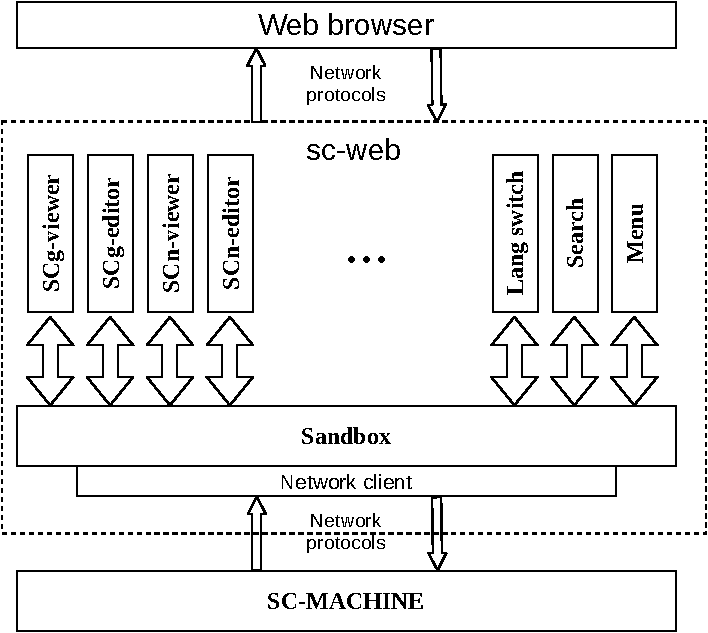
\includegraphics{figures/sd_interpreters/sc-web-new-arch.pdf}}}
\scnaddlevel{1}
	\scnexplanation{На данной иллюстрации показан планируемый вариант архитектуры \textit{Реализация интерпретатора sc-моделей пользовательских интерфейсов}, важным принципом которой является простота и однотипность подключения любых компонентов пользовательского интерфейса (редакторов, визуализаторов, переключателей, команд меню и т.д.). Для этого реализуется программная прослойка Sandbox, в рамках которой реализуются низкоуровневые операции взаимодействия с серверной частью и которая обеспечивает более удобный программный интерфейс для разработчиков компонентов.}
\scnaddlevel{-1}
\scnrelfromset{недостатки текущей реализации}{\scnfileitem{Отсутствие единого унифицированного механизма клиент-серверного взаимодействия. Часть компонентов (визуализатор sc-текстов в SCn-коде, команды меню и др.) работают по протоколу HTTP, часть по протоколу SCTP с использованием технологии WebSocket, это приводит к значительным трудностям при развитии платформы.};
\scnfileitem{Протокол HTTP предполагает четкое разделение активного клиента и пассивного сервера, который отвечает на запросы клиентов. Таким образом, сервер (в данном случае -- sc-память) практически не имеет возможности по своей инициативе отправить сообщение клиенту, что повышает безопасность системы, но значительно снижает ее интерактивность. Кроме того, такой вариант реализации затрудняет реализацию принятого в Технологии OSTIS многоагентного подхода, в частности, затрудняет реализацию sc-агентов на стороне клиента. Указанные проблемы могут быть решены путем постоянного мониторинга определенных событий со стороны клиента, однако такой вариант неэффективен.
Кроме того, часть интерфейса фактически работает напрямую с sc-памятью с использованием технологии WebSocket, а часть -- через прослойку на базе библиотеки tornado для языка программирования Python, что приводит к дополнительным зависимостям от сторонних библиотек.};
\scnfileitem{Часть компонентов (например, поле поиска по идентификатору) реализована сторонними средствами и практически никак не связана с sc-памятью. Это затрудняет развитие платформы.};
\scnfileitem{Текущая \textit{Реализация интерпретатора sc-моделей пользовательских интерфейсов} ориентирована только на ведение диалога с пользователем (в стиле вопрос пользователя -- ответ системы). Не поддерживаются такие очевидно необходимые ситуации, как выполнение команды, не предполагающей ответа\char59~возникновение ошибки или отсутствие ответа\char59~необходимость задания вопроса системой пользователю и т.д.};
\scnfileitem{Ограничена возможность взаимодействия пользователя с системой без использования специальных элементов управления. Например, можно задать вопрос системе, нарисовав его в SCg-коде, но ответ пользователь не увидит, хотя в памяти он будет сформирован соответствующим агентом.;
Большая часть технологий, использованных при реализации платформы, к настоящему моменту устарела, что затрудняет развитие платформы.};
\scnfileitem{Идея платформенной независимости пользовательского интерфейса (построения sc-модели пользовательского интерфейса) реализована не в полной мере. Полностью описать sc-модель пользовательского интерфейса (включая точное размещение, размеры, дизайн компонентов, их поведение и др.) в настоящее время скорее всего окажется затруднительно из-за ограничений производительности, однако вполне возможно реализовать возможность задания вопросов ко всем компонентам интерфейса, изменить их расположение и т.д., однако эти возможности нельзя реализовать в текущей версии реализации платформы.};
\scnfileitem{Интерфейсная часть работает медленно из-за недостатков  протокола SCTP и некоторых недостатков реализации серверной части на языке Python.};
\scnfileitem{Не реализован механизм наследования при добавлении новых внешних языков. Например, добавление нового языка даже очень близкого к SCg-коду требует физического копирования кода компонента и внесение соответствующих изменений, при этом получаются два никак не связанных между собой компонента, которые начинают развиваться независимо друг от друга.};
\scnfileitem{Слабый уровень задокументированности текущей \textit{Реализации интерпретатора sc-моделей пользовательских интерфейсов}.}}
\scnrelfromset{требования к будущей реализации}{\scnfileitem{Унифицировать принципы взаимодействия всех компонентов интерфейса с \textit{Программной моделью sc-памяти}, независимо от того, к какому типу относится компонент. Например, список команд меню должен формироваться через тот же механизм, что и ответ на запрос пользователя, и команда редактирования, сформированная пользователем, и команда добавления нового фрагмента в базу знаний и т.д.};
\scnfileitem{Унифицировать принципы взаимодействия пользователей с системой независимо от способа взаимодействия и внешнего языка. Например, должна быть возможность задания вопросов и выполнения других команд прямо через SCg/SCn интерфейс. При этом необходимо учитывать принципы редактирования базы знаний, чтобы пользователя не мог под видом задания вопроса внести новую информацию в согласованную часть базы знаний.};
\scnfileitem{Унифицировать принципы обработки событий, происходящих при взаимодействии пользователя с компонентами интерфейса -- поведение кнопок и других интерактивных компонентов должно задаваться не статически сторонними средствами, а реализовываться в виде агента, который, тем не менее, может быть реализован произвольным образом (не обязательно на платформенно-независимом уровне). Любое действие, совершаемое пользователем, на логическом уровне должно трактоваться и обрабатываться как инициирование агента.};
\scnfileitem{Обеспечить возможность выполнять команды (в частности, задавать вопросы) с произвольным количеством аргументов, в том числе -- без аргументов.};
\scnfileitem{Обеспечить возможность отображения ответа на вопрос по частям, если ответ очень большой и для отображения требуется много времени.};
\scnfileitem{Каждый отображаемый компонент интерфейса должен трактоваться как изображение некоторого sc-узла, описанного в базе знаний. Таким образом, пользователь должен иметь возможность задания произвольных вопросов к любым компонентам интерфейса.};
\scnfileitem{Максимально упростить и задокументировать механизм добавления новых компонентов.};
\scnfileitem{Обеспечить возможность добавления новых компонентов на основе имеющихся без создания независимых копий. Например, должна быть возможность создать компонент для языка, расширяющего язык SCg новыми примитивами, переопределять принципы размещения sc-текстов и т.д.};
\scnfileitem{Свести к минимуму зависимость от сторонних библиотек.};
\scnfileitem{Свести к минимуму использование протокола HTTP (начальная загрузка общей структуры интерфейса), обеспечить возможность равноправного двустороннего взаимодействия серверной и клиентской части.};
\scnfileitem{Полностью отказаться от протокола SCTP, перейти на протокол на базе JSON, задокументировать его.}}
\scnaddlevel{1}
	\scnnote{Очевидно, что реализация большинства из приведенных требований связана не только с собственно вариантом реализации платформы, но и требует развития теории логико-семантических моделей пользовательских интерфейсов и уточнения в рамках нее общих принципов организации пользовательских интерфейсов ostis-систем. Однако, принципиальная возможность реализации таких моделей должна быть учтена в рамках реализации платформы.}
\scnaddlevel{-1}
\scnrelfromlist{компонент программной системы}{Панель меню команд пользовательского интерфейса\\
	\scnaddlevel{1}
		\scnexplanation{\textit{Панель меню команд пользовательского интерфейса} содержит изображения классов команд (как атомарных, так и неатомарных), имеющихся на данный момент в базе знаний и входящих в декомпозицию \textit{Главного меню пользовательского интерфейса} (имеется в виду полная декомпозиция, которая в общем случае может включать несколько уровней неатомарных классов команд).\\
		Взаимодействие с изображением неатомарного класса команд инициирует команду изображения классов команд, входящих в декомпозицию данного неатомарного класса команд.\\
		Взаимодействие с изображением атомарного класса команд инициирует генерацию команды данного класса с ранее выбранными аргументами на основе соответствующей \textit{обобщенной формулировки класса команд} (шаблона класса команд).}
	\scnaddlevel{-1}
	;Компонент переключения языка идентификации отображаемых sc-элементов\\
	\scnaddlevel{1}
		\scnexplanation{\textit{Компонент переключения языка идентификации отображаемых sc-элементов} является изображением множества имеющихся в системе естественных языков. Взаимодействие пользователя с данным компонентом переключает пользовательский интерфейс в режим общения с конкретным пользователем с использованием \textit{основных sc-идентификаторов}, принадлежащих данному \textit{естественному языку}. Это значит, что при изображении sc-идентификаторов sc-элементов на каком-либо языке, например, SCg-коде или SCn-коде будут использоваться \textit{основные sc-идентификаторы}, принадлежащие данному \textit{естественному языку}. Это касается как sc-элементов, отображаемых в рамках \textit{Панели визуализации и редактирования знаний}, так и любых других sc-элементов, например, классов команд и даже самих \textit{естественных языков}, изображаемых в рамках самого \textit{Компонента переключения языка идентификации отображаемых sc-элементов}.}
	\scnaddlevel{-1}	
	;Компонент переключения внешнего языка визуализации знаний\\
	\scnaddlevel{1}
		\scnexplanation{\textit{Компонент переключения внешнего языка визуализации знаний} служит для переключения языка визуализации знаний в текущем окне, отображаемом на \textit{Панели визуализации и редактирования знаний}. В текущей реализации в качестве таких языков по умолчанию поддерживаются SCg-код и SCn-код, а также любые другие языки, входящие во множество \textit{внешних языков визуализации SC-кода}.}
	\scnaddlevel{-1}
	;Поле поиска sc-элементов по идентификатору\\
	\scnaddlevel{1}
		\scnexplanation{\textit{Поле поиска sc-элементов по идентификатору} позволяет осуществлять поиск sc-идентификаторов, содержащих подстроку, введенную в данное поле (с учетом регистра). В результате поиска отображается список sc-идентификаторов, содержащих указанную подстроку, при взаимодействии с которыми осуществляется автоматическое задание вопроса ``Что это такое?'', аргументом которого является либо для сам sc-элемент, имеющий данный sc-идентификатор (в случае, если указанный sc-идентификатор является основным или системным, и, таким образом, указанный sc-элемент может быть определен однозначно), либо для самого внутреннего файла ostis-системы, являющегося sc-идентификатором (в случае, если данный sc-идентификатор является неосновным).}
	\scnaddlevel{-1}
	;Панель отображения диалога пользователя с ostis-системой\\
	\scnaddlevel{1}
		\scnexplanation{\textit{Панель отображения диалога пользователя с ostis-системой} отображает упорядоченный по времени список sc-элементов, являющихся знаками действий, которые инициировал пользователь в рамках диалога с ostis-системой путем взаимодействия с изображениями соответствующих классов команд (то есть, если действие было инициировано другим способом, например, путем его явного инициирования через создание дуги принадлежности множеству \textit{инициированных действий} в sc.g-редакторе, то на данной панели оно отображено не будет). При взаимодействии пользователя с любым из изображенных знаков действий на \textit{Панели визуализации и редактирования знаний} отображается окно, содержащее результат выполнения данного \textit{действия} на том языке визуализации, на котором он был отображен, когда пользователь просматривал его в последний (предыдущий) раз. Таким образом, в текущей реализации данная панель может работать только в том случае, если инициированное пользователем действие предполагает явно представленный в памяти результат данного действия. В свою очередь, из этого следует, что в настоящее время данная панель, как и в целом \textit{Реализация интерпретатора sc-моделей пользовательских интерфейсов}, позволяет работать с системой только в режиме диалога ''вопрос-ответ''.}
	\scnaddlevel{-1}
	;Панель визуализации и редактирования знаний\\
	\scnaddlevel{1}
		\scnexplanation{\textit{Панель визуализации и редактирования знаний} отображает окна, содержащие sc-текст, представленный на некотором языке из множества \textit{внешних языков визуализации SC-кода} и, как правило, являющийся результатом некоторого действия, инициированного пользователем. Если соответствующий визуализатор поддерживает возможность редактирования текстов соответствующего естественного языка, то он одновременно является также и редактором.}
		\scnrelfromlist{компонент программной системы}{Визуализатор sc.n-текстов;Визуализатор и редактор sc.g-текстов}
		\scnnote{При необходимости пользовательский интерфейс каждой конкретной ostis-системы может быть дополнен визуализаторами и редакторами различных внешних языков, которые в текущей версии \textit{Реализации интерпретатора sc-моделей пользовательских интерфейсов} будут также располагаться на \textit{Панели визуализации и редактирования знаний}.}
	\scnaddlevel{-1}}

\scnheader{Реализация scp-интерпретатора}
\scnrelto{программная реализация}{Абстрактная scp-машина}
\scnnote{Важнейшей особенностью Языка SCP является тот факт, что его программы записываются таким же образом, что и обрабатываемые ими знания, то есть в SC-коде. Это, с одной стороны, дает возможность сделать ostis-системы платформенно-независимыми (четко разделить \textit{sc-модель компьютерной системы} и платформу интерпретации таких моделей), а с другой стороны требует наличия в рамках платформы \textit{Реализации scp-интерпретатора}, то есть интерпретатора программ Языка SCP.}
\scnrelfromlist{используемый язык программирования}{C++}
\scnrelfromlist{компонент программной системы}{Реализация Абстрактного sc-агента создания scp-процессов;Реализация Абстрактного sc-агента интерпретации scp-операторов\\
	\scnaddlevel{1}
	\scnrelfromlist{компонент программной системы}{Реализация Абстрактного sc-агента интерпретации scp-операторов генерации конструкций;Реализация Абстрактного sc-агента интерпретации scp-операторов ассоциативного поиска конструкций;Реализация Абстрактного sc-агента интерпретации scp-операторов удаления конструкций;Реализация Абстрактного sc-агента интерпретации scp-операторов проверки условий;Реализация Абстрактного sc-агента интерпретации scp-операторов управления значениями операндов;Реализация Абстрактного sc-агента интерпретации scp-операторов управления scp-процессами;Реализация Абстрактного sc-агента интерпретации scp-операторов управления событиями;Реализация Абстрактного sc-агента интерпретации scp-операторов обработки содержимых числовых файлов;Реализация Абстрактного sc-агента интерпретации scp-операторов обработки содержимых строковых файлов}
	\scnaddlevel{-1}
	;Реализация Абстрактного sc-агента синхронизации процесса интерпретации scp-программ;Реализация Абстрактного sc-агента уничтожения scp-процессов;Реализация Абстрактного sc-агента синхронизации событий в sc-памяти и ее реализации}
\scnnote{Текущая \textit{Реализация scp-интерпретатора} не включает в себя специализированных средств для работы с блокировками, поскольку механизм блокировок элементов sc-памяти реализован на более низком уровне в рамках \textit{Реализация sc-хранилища и механизма доступа к нему}}

\scnendstruct \scnendcurrentsectioncomment

\end{SCn}